%!TEX root = main.tex
% UTF-8 encoding

\section{Related Work}
\label{sec:related_work}
Natural language processing (NLP) 
has been used effectively in various security and privacy problems, including clustering illicit online pharmacies \cite{leontiadis2011measuring,mccoy2012pharmaleaks}, identifying sensitive user inputs \cite{huang2015supor,nan2015uipicker}, and detecting spam \cite{thomas2013trafficking,sedhai2017semi,wu2018twitter,wu2017twitter}. 
% Here, we focus its use in analyzing euphemisms.  
However, although euphemisms have been widely studied in linguistics and related disciplines  \cite{keith1991euphemism,pfaff1997metaphor,hugh2002rawson,allan2009connotations,rababah2014translatability,spears1981slang,chilton1987metaphor,ahl2006motivation,fernandez2006language}, they have  received relatively little attention from the NLP \cite{felt2020recognizing}, or security and privacy communities. 
Next, we review relevant prior work, including: 1) euphemism detection, %(in Section \ref{sec:related_det}) 
2) euphemism identification, and 3) self-supervised learning. % (in Section \ref{sec:related_iden}). 


\subsection{Euphemism Detection}
\label{sec:related_det}

\begin{table*}[t!]
	\centering
	\small
	\caption{Related work on euphemism detection.}
	\begin{tabular}{p{0.10\textwidth}p{0.12\textwidth}p{0.22\textwidth}p{0.22\textwidth}p{0.22\textwidth}}
		\toprule
		\centering{\textbf{System}} & \centering{\textbf{Learning Type}} & \centering{\textbf{Categories (Platform)}} & \centering{\textbf{Required Input}} & \multicolumn{1}{c}{\textbf{Approach Keywords}} \\
		\midrule
		\textbf{Durrett \etal (2017) \cite{durrett2017identifying}} & Supervised \& semi-supervised  & Cybercriminal wares (Darkode), cybersecurity (Hack Forums), search engine optimization techniques (Blackhat), data stealing tools and services (Nulled) & A fully labelled dataset with annotated euphemisms & Cross-domain, Support Vector Machine (SVM), Conditional Random Field (CRF) \\
		%\midrule
		\\ 
		\textbf{Pei \etal (2019) \cite{pei2019slang}} & Supervised  & General topics (Online Slang Dictionary)  & Slang-less corpus (Penn Treebank) as the negative examples, Slang-specific corpus (Online Slang Dictionary) as the positive examples & Linguistic features, bidirectional LSTM \cite{huang2015bidirectional} , Conditional Random Field (CRF) \cite{lafferty2001conditional}, multilayer perceptron (MLP) \cite{rauber2011kernel} \\ 
		%\midrule	
		\\
		\textbf{Zhao \etal (2016) \cite{zhao2016chinese}} & Unsupervised  & Cybersecurity (QQ) & Target keywords, online search service & Unsupervised learning, word embedding (\ie, word2vec), Latent Dirichlet Allocation (LDA) \\
		%\midrule
		\\
		\textbf{Yang \etal (2017) \cite{yang2017learn}} & Unsupervised  & Sex, gambling, dangerous goods, surrogacy, drug, faked sites (Baidu) & Target keywords, online search service & Web analysis, keywords expansion, candidate filtering\\
		%\midrule
		\\
		\textbf{Takuro \etal (2020) \cite{takuro2020codewords}} & Unsupervised & Drug trafficking and enjo kosai (Twitter) & A clean background corpus, a bad corpus related to illegal transactions, a set of euphemism seeds & Word embedding (word2vec), cosine similarity \\
		%\midrule
		\\
		\textbf{Felt \etal (2020) \cite{felt2020recognizing}} & Unsupervised & Firing, lying and stealing (The English Gigaword corpus) & Category name, a lexicon dictionary (\ie, Gigaword) & Sentiment analysis, bootstrapping, semantic lexicon induction \\
		%\midrule
		\\
		\textbf{Taylor \etal (2017) \cite{taylor2017surfacing}} & Unsupervised &  Hate speech (Twitter) &  The text corpus, category name & Word embedding (fasttext \cite{bojanowski2017enriching} and dependency2vec \cite{levy2014dependency}), community detection, bootstrapping \\
		%\midrule
		\\
		\textbf{Magu \etal (2018) \cite{magu2018determining}} & Unsupervised &  Hate speech (Twitter) & The text corpus, a euphemism seed & Word embedding (word2vec), network analysis, centrality measures \\
		%\midrule
		\\
		\textbf{Yuan \etal (2018) \cite{yuan2018reading}} & Unsupervised & Sale and trade of hacking services and tools (Darkode), blackhat hacking (Hack Forums), data stealing tool and service (Nulled), illegal drug (Silk Road) & A background corpus (\eg, Wikipedia), A dark corpus (\eg, Silk Road \cite{christin2013traveling}), A mixed corpus (\eg, Reddit) & Word embedding, semantic comparison across corpora \\
		\midrule
		\textbf{Our algorithm} & Unsupervised & Drug (\ie, Reddit), weapon (\ie, Gab, SlangPedia, \cite{durrett2017identifying}), sexuality (\ie, Gab) & The text corpus, target keywords & Contextual information, masked language model, BERT \\
		\bottomrule
	\end{tabular}
	\label{table:related_dec}
\end{table*}



Euphemism detection is broadly related to the tasks of set expansion \cite{shen2017setexpan,zhu2019fuse,zhang2020empower,huang2020guiding,shen2020synsetexpan,rong2016egoset} and lexicon construction and induction \cite{hamilton2016inducing,yang2020co,huang2020corel,mao2020octet,shang2020nettaxo,shen2020taxoexpan,zhang2018taxogen}. %, with the differences highlighted below. 
Set expansion aims to expand a small set of seed entities into a complete set of relevant entities, and its goal is to find other target keywords from the same category. 
Lexicon construction and induction focus on extracting relations and building the lexicon-based knowledge graph in a structured manner. 
Their  goals are different from ours, which is to find euphemisms of  target words. 


The specific task of euphemism detection has been studied in the NLP literature under a number of frameworks, including supervised, semi-supervised, and unsupervised learning, summarized in Table \ref{table:related_dec}.
% With regard to euphemism detection, a number of models have been proposed in supervised, semi-supervised and unsupervised learning scheme, on diverse categories and platforms, with and without distant-supervisions, as summarized in Table \ref{table:related_dec}. 
For example, Yang et al.\ \cite{yang2017learn} build a  Keyword Detection and Expansion System (KDES) and apply it to the search results of Baidu, China's top search engine. 
KDES aims to infer whether a search keyword should be blocked by inspecting the associated search results.
% and using related search queries to extend the findings.
This approach requires general domain information with distant-supervision (\ie, the Baidu search engine), and is therefore not suitable for our unsupervised setting. % discovering euphemism detection in a given text corpus. 
Even if assuming search engine access, 
euphemisms for sensitive keywords are often short and innocent-looking (\eg, blueberries), 
which may result in mainly legitimate search results. 
Another set of relevant 
articles \cite{durrett2017identifying,portnoff2017tools} generate high-level information to analyze underground forums via an automated, 
top-down approach that blends information extraction and named-entity recognition. 
They present a data annotation method and utilize the labeled data to train a supervised learning-based
classifier. 
Yet, the results depend heavily on the quality of annotation, and as shown by several researchers \cite{durrett2017identifying,yuan2018reading}, the model does not perform as well in cross-domain datasets, 
where it is outperformed by standard  semi-supervised learning techniques. 
% To examine how recent deep learning models support automatic euphemism detection, \cite{pei2019slang} study a combination of bidirectional recurrent neural networks, conditional random fields, and multilayer perceptrons, and show that linguistic features combined with deep learning algorithms offer interpretability. 

\begin{figure*}[t]
	\centering
	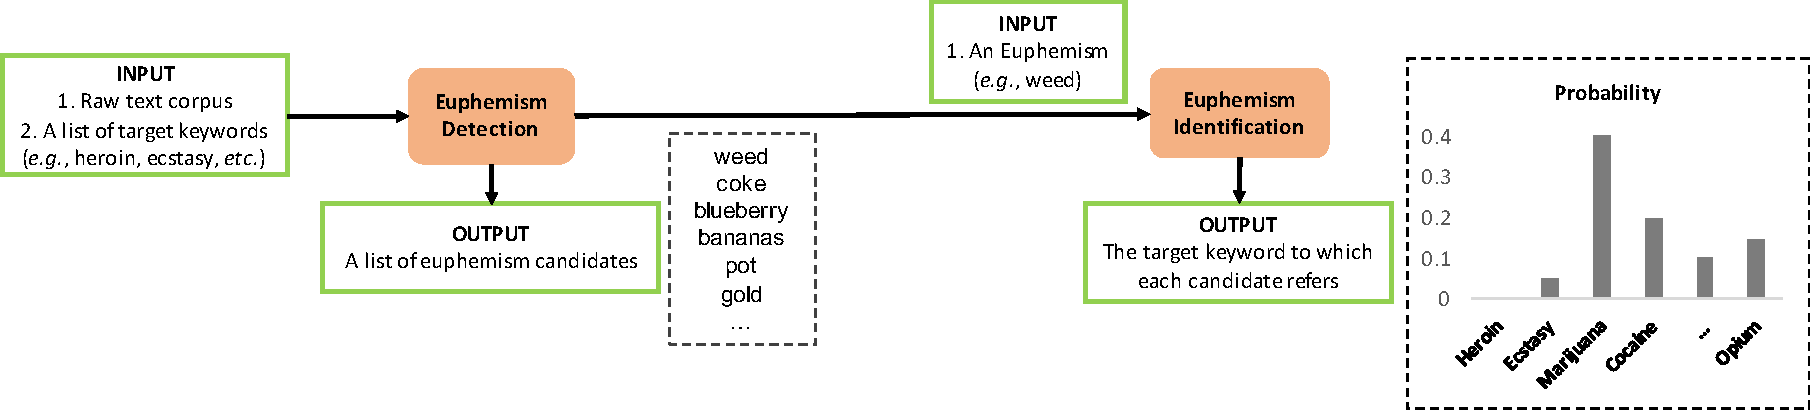
\includegraphics[width=1.00\linewidth]{figures/1}
	\caption{Euphemism detection and identification pipeline.}
	\label{fig:model_overview}
\end{figure*}

Our work is most closely related to four state-of-the-art approaches \cite{yuan2018reading,felt2020recognizing,taylor2017surfacing,magu2018determining}. 
CantReader \cite{yuan2018reading} aims to automatically identify ``dark jargon'' from cybercrime marketplaces. 
CantReader employs a neural-network based embedding technique to analyze the semantics of words, and detects euphemism candidates whose contexts in the background corpus (\eg, Wikipedia) are significantly different from those in the target corpus. 
Therefore, it takes as input a ``dark'' corpus (\eg, Silk Road anonymous online marketplace \cite{christin2013traveling} forum), a mixed corpus (\eg, Reddit), and a benign corpus (\eg, English Wikipedia). 
Different from CantReader, 
we assume only access to a single target corpus -- although we do rely on context-aware embeddings that could be pre-trained from a reference corpus like Wikipedia, and then fine-tuned to the target corpus.
More importantly, we find that our approach outperforms CantReader, presumably because we explicitly use context.
%does not achieve performance competitive with ours, presumably due to the fact that it does not make explicit use of context. 

Another relevant baseline \cite{felt2020recognizing} detects euphemisms instead by using sentiment analysis. 
It identifies a set of  euphemism candidates using a bootstrapping algorithm for semantic lexicon induction. 
Though the methodology seems reasonable and intuitive at first, it requires additional manual filtering process to refine the candidates and thus, fails to meet the requirement of automatic, large-scale detection 
that online content moderators desire. 
In yet another approach, Magu et al.\ \cite{magu2018determining} and Taylor et al.\ \cite{taylor2017surfacing} propose two algorithms that leverage word embeddings and community detection algorithms. 
Magu et al.\ \cite{magu2018determining} generates a cluster of euphemisms by the ranking metric of eigenvector centralities \cite{bonacich1972factoring,bonacich1972technique}.
Due to the intrinsic nature of the algorithm, this approach 
requires a starting euphemism seed to find others. 
Taylor et al.\ \cite{taylor2017surfacing} creates neural embedding models that capture the word similarities, uses graph expansion and the PageRank scores \cite{page1999pagerank} to bootstrap initial seed words, and finally enriches the bootstrapped words to learn out-of-dictionary terms that behave like euphemisms.
However, the approaches of Magu et al.\ \cite{magu2018determining} and Taylor et al.\ \cite{taylor2017surfacing} were tested on a single dataset.  
Unfortunately, 
we do not find their performance to be as strong on the multiple datasets we evaluate. 

%and we find their performance to be poor on all of  the datasets we evaluated.
% calling into question its effectiveness for other datasets and categories. 





\subsection{Euphemism Identification}
\label{sec:related_iden}
To the best of our knowledge, no work has explicitly attempted to infer euphemism meaning.
% except for a few peripheral works that identify the broad category of a euphemism. 
Yuan et al.\ \cite{yuan2018reading} tackles a related problem by identifying the hypernym of euphemisms (\eg, whether it refers to a drug or a person).
% It first extracts a set of hypernym candidates, and then run a classifier to determine the best candidate to serve as the hypernym of a euphemism. 
In a more general sense, the task of euphemism identification is also related to sense discovery of unknown words \cite{ishiwatari2019learning,ni2017learning} and word sense disambiguation \cite{taghipour2015semi,raganato2017neural,raganato2017word,iacobacci2016embeddings}. 
Sense discovery aims to understand the meaning of an unknown word by generating a definition sentence. 
Word sense disambiguation focuses on identifying which sense of a word is used in a sentence, given a set of candidate senses.
% and It is typically a form of multiple choice questions with distinct sense meanings. 
However, neither of these are able to capture nuanced differences between a group of semantically-similar target words in the same category. 

\subsection{Self-supervised Learning}
The technical innovations in our 
work rely heavily on  \emph{self-supervision}, a form of unsupervised learning where the data itself provides the supervision \cite{weng2019selfsup}. 
% We achieve euphemism identification by proposing a self-supervised learning algorithm, a form of unsupervised learning where the data itself provides the supervision \cite{weng2019selfsup}. 
% Below, we provide some background of self-supervised learning and review some important ideas and works. 
%\noindent \textbf{Self-supervised learning}: 
% Given a task and enough labels, supervised learning can typically solve it really well. 
% Supervised learning requires labelled data (\eg, ImageNet), which is expensive to obtain. %  and hard to be scaled up. 
Self-supervision was designed to make use of vast amounts of unlabelled data (\eg, free text, images) 
by constructing a supervised learning task from the data itself to predict some attribute of the data.
For example, to train a text prediction model, one can take a corpus of text, mask part of the sentence, and train the model to predict the masked part;
this workflow creates a supervised learning task from unlabelled data.
% An example might be to modify training samples in a controlled fashion and train a sub-model to identify the modification.
% The nature of the self-supervised task typically depends on the application. 
% For example, suppose we are training an image classifier and have only , we could train our model on modified 
% is substantially more than a limited number of human curated labelled datasets, it is wasteful not to use them. However, unsupervised learning is not easy and usually works much less efficiently than supervised learning.
%What if we can get labels for free for unlabelled data and train unsupervised dataset in a supervised manner? We can achieve this by framing a supervised learning task in a special form to predict only a subset of information using the rest. In this way, all the information needed, both inputs and labels, has been provided. This is known as self-supervised learning.
Self-supervision has been widely used in language modeling \cite{devlin2019bert,lan2019albert,liu2019roberta,baevski2020wav2vec,chen2020big,liu2018empower}, representation learning \cite{feng2019self,kolesnikov2019revisiting,sabokrou2019self}, robotics \cite{mees2019self,nair2017combining,berscheid2020self}, computer vision \cite{zhai2019s4l,sun2019unsupervised,xu2019self,yin2020dreaming} and reinforcement learning \cite{kahn2018self,zeng2018learning,pong2019skew}. 
One of our contributions is to generalize and extend the idea of self-supervision to the task of euphemism identification. 


% Self-supervised learning empowers us to exploit a variety of labels that come with the data for free. The motivation is quite straightforward. Producing a dataset with clean labels is expensive but unlabeled data is being generated all the time. To make use of this much larger amount of unlabeled data, one way is to set the learning objectives properly so as to get supervision from the data itself.


